\section{约束问题}
\label{sec:kkt-problem}

把“带约束的最小化”固定成全章共用的形式，并看清边界上的最优点与无约束最优点到底差在哪里？先从预算分配的例子开始。

\paragraph{预算分配}
设两项开支的金额为$\bm{x}=(x_1,x_2)$，金额不能为负，总额不能超过预算$\tau$。理想的分配是$\bm{c}=(2,1)$，我们用平方距离衡量偏离理想的程度，于是要解
\begin{equation}
 \min_{x_1,x_2}\ \frac12\bigl[(x_1-2)^2+(x_2-1)^2\bigr]
 \quad\text{s.t.}\quad x_1+x_2\leq\tau,\ x_1\geq0,\ x_2\geq0.
 \label{eq:kkt-budget}
\end{equation}
目标的等高线是以$\bm{c}$为圆心的同心圆。可行集是直角边长为$\tau$的三角形。问题问的是：三角形里哪一点离$\bm{c}$最近？

取$\tau=2$。此时$c_1+c_2=3>2$，$\bm{c}$在三角形之外。圆从$\bm{c}$开始逐渐胀大，第一次碰到三角形的位置就是最优点。这一点是$\bm{c}$到直线$x_1+x_2=2$的垂足，把$\bm{c}$沿法向$(1,1)$退回去就得到：
\[
 \bm{x}^\star=\bm{c}-\frac{3-2}{2}(1,1)=\Bigl(\frac32,\frac12\Bigr).
\]

这个几何答案也可以用不等式直接验证。令$a=2-x_1$，$b=1-x_2$，可行点满足$a+b=3-x_1-x_2\geq1$。由$a^2+b^2\geq(a+b)^2/2$，得到
\[
 f(\bm{x})=\frac12(a^2+b^2)\geq\frac14(a+b)^2\geq\frac14.
\]
等号成立当且仅当$a=b=1/2$，也就是$\bm{x}=(3/2,1/2)$，这一点可行，所以最优值是$1/4$。这种配方只对这一个例子管用，本章要找的是能照章执行的判别方法。

现在看最优点处的梯度：
\[
 \nabla f(\bm{x}^\star)=\bm{x}^\star-\bm{c}=\Bigl(-\frac12,-\frac12\Bigr)\neq\bm{0}.
\]
负梯度$(1/2,1/2)$指向$\bm{c}$，沿它走目标确实下降，但它穿出了预算线。图~\ref{fig:kkt-budget-boundary}中，蓝色箭头所指的方向就是目标“想去”却去不了的地方。这是边界最优的典型样子：梯度不为零，只是所有下降方向都被约束挡住了。

\begin{BookInlineFigure}
  \centering
  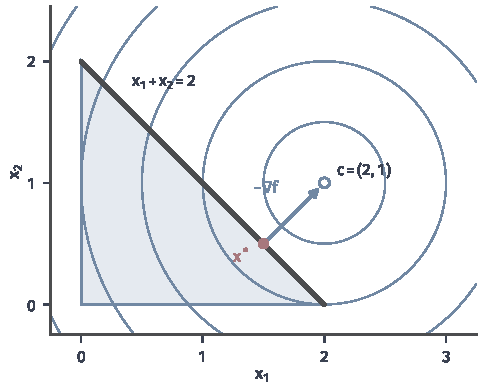
\includegraphics[width=82mm]{figures/05-optimization/06-constrained-optimization/matplotlib/kkt-budget-boundary/figure.pdf}
  \caption{预算分配（$\tau=2$）的边界最优点。浅蓝三角形是可行集，蓝色圆是目标$\frac12\lVert\bm{x}-\bm{c}\rVert_2^2$的等高线，空心点是不可行的理想分配$\bm{c}=(2,1)$，深灰粗线是起作用的预算线。红点$\bm{x}^\star=(3/2,1/2)$处，负梯度（蓝色箭头）非零，指向可行集外。}
  \label{fig:kkt-budget-boundary}
\end{BookInlineFigure}

\paragraph{一般形式}
本章和本部分后面各章都讨论下面的问题。给定$\bm{x}\in\mathbb{R}^n$的目标函数$f$、不等式约束函数$g_1,\ldots,g_m$和等式约束函数$h_1,\ldots,h_p$，求解
\begin{equation}
 \begin{aligned}
  \min_{\bm{x}\in\mathbb{R}^n}\quad&f(\bm{x})\\
  \text{s.t.}\quad&g_i(\bm{x})\leq0,\quad i=1,\ldots,m,\\
  &h_j(\bm{x})=0,\quad j=1,\ldots,p.
 \end{aligned}
 \label{eq:kkt-problem}
\end{equation}
可行集记为
\begin{equation}
 \bm{C}=\{\bm{x}\in\mathbb{R}^n:g_i(\bm{x})\leq0,\ i=1,\ldots,m;\ h_j(\bm{x})=0,\ j=1,\ldots,p\}.
 \label{eq:kkt-feasible}
\end{equation}

除非另有说明，假设$f$、$g_i$、$h_j$都定义在包含$\bm{C}$的开集上，并且连续可微；讨论二阶条件时再要求二阶连续可微。所有不等式都整理成“$\leq0$”，这个约定决定了后面乘子的符号。预算分配写成这种形式，三个不等式约束是
\begin{equation}
 g_1(\bm{x})=x_1+x_2-\tau,\qquad g_2(\bm{x})=-x_1,\qquad g_3(\bm{x})=-x_2.
 \label{eq:kkt-budget-constraints}
\end{equation}
它们的梯度依次是常向量$(1,1)$、$(-1,0)$、$(0,-1)$，都指向使约束函数增大的一侧，也就是可行集的外侧。

\paragraph{活动约束}
站在一个可行点$\bar{\bm{x}}$上，不等式约束分成两类。若$g_i(\bar{\bm{x}})=0$，这条约束正好卡在边界上，稍有不慎就会违反，称它在$\bar{\bm{x}}$处是\term{活动约束}（active constraint）。若$g_i(\bar{\bm{x}})<0$，$g_i$是连续函数，所以在$\bar{\bm{x}}$的某个邻域内仍有$g_i<0$，这条约束在局部不起任何限制作用。活动约束的下标集记为
\begin{equation}
 A(\bar{\bm{x}})=\{i\in\{1,\ldots,m\}:g_i(\bar{\bm{x}})=0\},
 \label{eq:kkt-active-set}
\end{equation}
称为\term{活动集}（active set）。等式约束总在起作用，但$A(\bar{\bm{x}})$只记不等式的下标。

图~\ref{fig:kkt-active-sets}取$\tau=2$，看三个可行点。内部点$(0.6,0.6)$没有活动约束，四周都能走。预算线上的点$(3/2,1/2)$只有$g_1$活动，能走的方向少了一半。角点$(2,0)$处$g_1$与$g_3$同时活动，能走的方向只剩一个楔形。虚线圆是一个小邻域，圆内真正影响移动的只有粗线。

\begin{BookInlineFigure}
  \centering
  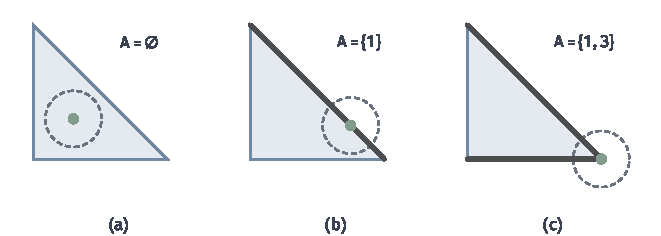
\includegraphics[width=112mm]{figures/05-optimization/06-constrained-optimization/matplotlib/kkt-active-sets/figure.pdf}
  \caption{预算三角形（$\tau=2$）中三个可行点的活动集。深灰粗线是该点的活动约束，虚线圆是一个小邻域。(a)内部点$(0.6,0.6)$没有活动约束。(b)预算线上的点$(3/2,1/2)$只有$g_1$活动。(c)角点$(2,0)$处$g_1$、$g_3$同时活动。}
  \label{fig:kkt-active-sets}
\end{BookInlineFigure}

\paragraph{局部与全局最小点}
第~\ref{chap:optimization}章区分了局部与全局最优解，本章沿用这两个概念，并按习惯称最优解为最小点。称可行点$\bm{x}^\star$是\term{局部最小点}（local minimizer），如果存在$r>0$，使
\begin{equation}
 f(\bm{x}^\star)\leq f(\bm{x})\quad\text{对所有}\ \bm{x}\in\bm{C},\ \lVert\bm{x}-\bm{x}^\star\rVert_2<r.
 \label{eq:kkt-local-min}
\end{equation}
若对$\bm{x}\neq\bm{x}^\star$不等式都严格成立，就称为严格局部最小点。要是式~\eqref{eq:kkt-local-min}对所有$\bm{x}\in\bm{C}$成立，$\bm{x}^\star$就是全局最小点。

比较只在可行点之间进行，所以邻域外和可行集外的点都不参加比较。下面的例子可以看出局部和全局的差别，而这两种点都可以落在边界上。在平面上最小化$f(\bm{x})=x_1$，约束是
\[
 g(\bm{x})=(x_2^2-1)^2+0.3\,x_2-x_1\leq0.
\]
可行集的左边界是一条弯曲的曲线，它有两个向左伸的凸起。

图~\ref{fig:kkt-local-global}中，每个凸起的顶点都比附近的可行点更靠左，因此都是局部最小点。解一元方程求边界曲线的极小，得到上方顶点约为$(0.294,0.960)$，下方顶点约为$(-0.305,-1.036)$，后者才是全局最小点。两处的梯度都等于$(1,0)$，并不为零。站在局部最小点上，只看附近无从知道下方还有更低的点，所以局部信息最多只能回答局部问题。

\begin{BookInlineFigure}
  \centering
  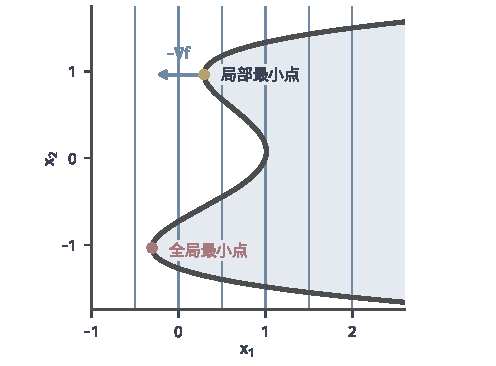
\includegraphics[width=84mm]{figures/05-optimization/06-constrained-optimization/matplotlib/kkt-local-global/figure.pdf}
  \caption{边界上的局部最小点与全局最小点。目标$f(\bm{x})=x_1$的等高线是竖直的蓝线，浅蓝区域是可行集$x_1\geq(x_2^2-1)^2+0.3x_2$，深灰粗线是边界。黄点是局部最小点，红点是全局最小点，两点的负梯度（蓝色箭头）都指向可行集外。}
  \label{fig:kkt-local-global}
\end{BookInlineFigure}

判断最优性时，本章要回答三个不同的问题：局部最小点必须满足什么（必要条件）？满足什么就一定是局部最小点（局部充分条件）？什么时候局部信息足以断定全局最优？解的存在性由第~\ref{chap:optimization}章的结论负责，例如预算三角形是非空紧集，目标连续，最优解一定存在。
